\documentclass[12pt,a4paper]{article}

\usepackage[margin=1in]{geometry}
\usepackage{setspace}
\usepackage{enumitem}
\usepackage{titlesec}
\usepackage{hyperref}
\usepackage{graphicx}
\usepackage{array}
\usepackage{longtable}
\usepackage{booktabs}
\usepackage{xcolor}
\usepackage{tikz}
\usetikzlibrary{arrows.meta,positioning,shapes.geometric}

\setstretch{1.15}
\setlength{\parindent}{0pt}
\setlength{\parskip}{6pt}

\titleformat{\section}{\large\bfseries}{\thesection.}{0.5em}{}
\titleformat{\subsection}{\normalsize\bfseries}{\thesubsection}{0.5em}{}

\begin{document}

\begin{center}
    {\LARGE \textbf{SYNOPSIS}}\\[0.5cm]
    {\Large \textbf{SmartRoad: Image-Based Road Condition Monitoring, Mapping and Repair Prioritization System}}
\end{center}

\section{Introduction}

Roads are an essential part of transportation infrastructure, but their condition gradually deteriorates because of heavy traffic, weather conditions, water accumulation, poor maintenance and regular wear and tear. Common problems such as potholes, cracks, damaged edges and uneven road surfaces can reduce driving comfort, damage vehicles and create safety risks.

Traditional road-condition monitoring mainly depends on manual inspection. Inspectors have to physically survey roads, identify defects and record their locations. This process can be time-consuming and difficult to repeat frequently over a large area. Sensor-based monitoring systems are another approach, but they may require additional hardware, installation and maintenance.

The proposed SmartRoad system uses photographs of roads instead of dedicated physical sensors. A photograph captured using a mobile phone, camera or an existing road-image dataset is provided as input. The system processes the image, identifies visible road defects, estimates their severity and associates the defect with a particular road/location.

The system further provides a 2D map-based view using \textbf{OpenStreetMap}. Interactive map functionality can be implemented using \textbf{Leaflet}. Defects can be marked on the map using different coloured markers. Green, yellow, orange and red markers can represent normal, moderate, high and critical road conditions respectively. This makes the condition of a road network easy to understand visually.

The project combines image processing with Data Structures and Algorithms in C, Object-Oriented Programming in C++, graph algorithms and GUI development to create a practical academic prototype.

\section{Problem Statement}

There is a need for a simple and cost-effective road-condition monitoring system that can use road photographs to identify visible defects and represent their locations on a real-world map.

The system should be able to:
\begin{enumerate}[leftmargin=*]
    \item Accept road photographs as input.
    \item Detect visible defects such as potholes and cracks.
    \item Classify defects according to type.
    \item Estimate the severity of each defect.
    \item Associate defects with exact road locations.
    \item Display road conditions on a 2D OpenStreetMap-based map.
    \item Store and manage defect information efficiently.
    \item Prioritize repair work according to severity.
    \item Suggest a suitable maintenance route.
\end{enumerate}

\section{Motivation}

The main motivation of this project is to make road-condition monitoring more accessible by using photographs rather than dedicated sensor hardware.

A road photograph contains visual information about the road surface. Image-processing techniques can be used to analyze this information and identify damaged regions. The detected information can then be converted into structured records and displayed on a map.

The project also provides a practical application of academic concepts. Queue, Linked List, Priority Queue and Graph are applied to actual system requirements. Similarly, OOP concepts such as abstraction, encapsulation, inheritance and polymorphism are used to model different road-defect types.

The map-based interface further improves the system because users can select the exact defect location on the OpenStreetMap-based interface and visually identify which roads require attention.

\section{Objectives}

\begin{enumerate}[leftmargin=*]
    \item To develop an image-based road-condition monitoring system.
    \item To use road photographs as the primary input instead of dedicated physical sensors.
    \item To detect visible road defects such as potholes, cracks and damaged regions.
    \item To classify detected defects according to their type.
    \item To estimate defect severity as Low, Medium, High or Critical.
    \item To associate detected defects with a particular road and exact map location.
    \item To display road conditions and defect markers on an OpenStreetMap-based 2D map.
    \item To implement Queue, Linked List and Priority Queue for efficient data management.
    \item To represent the road network using a Graph.
    \item To use Dijkstra's algorithm or A* for maintenance-route planning.
    \item To apply OOP concepts using C++.
    \item To provide a simple and user-friendly GUI dashboard.
\end{enumerate}

\section{Proposed System}

The SmartRoad system will work as an integrated image-analysis and map-based road-monitoring application.

First, the user selects a road photograph. The image is passed to the image-processing module, where basic preprocessing such as resizing, grayscale conversion, noise reduction, contrast enhancement and edge/region analysis may be performed.

The processed image is then analyzed to identify candidate damaged regions. Depending on the available dataset and implementation level, defect detection may be performed using image-processing rules, thresholding, contours/features or a lightweight trained model.

After detection, a \texttt{RoadDefect} object is created. Different defect types such as \texttt{Pothole}, \texttt{Crack} and \texttt{DamagedEdge} can be represented as derived classes of a common \texttt{RoadDefect} class.

Each defect can contain:
\begin{itemize}[leftmargin=*]
    \item Defect ID
    \item Defect type
    \item Severity
    \item Road name/ID
    \item Latitude and longitude
    \item Image reference/path
    \item Repair status
\end{itemize}

\subsection{Exact Location Association}

For the academic prototype, the simplest location method will be used: after uploading a photograph, the user can open the OpenStreetMap-based map and \textbf{click on the exact location of the defect}. The application records the latitude and longitude of the selected point.

For example:

\begin{verbatim}
Defect ID   : 101
Image       : road_01.jpg
Type        : Pothole
Severity    : High
Latitude    : 30.342156
Longitude   : 78.065421
Status      : Pending
\end{verbatim}

The defect ID is linked to the complete \texttt{RoadDefect} record. The record contains both the image reference and the map coordinates. Therefore, clicking the corresponding map marker can display the defect details and the associated photograph.

This approach does not require the photograph itself to contain GPS metadata. Automatic GPS/EXIF extraction can be considered as a future enhancement.

\section{System Workflow}

\begin{center}
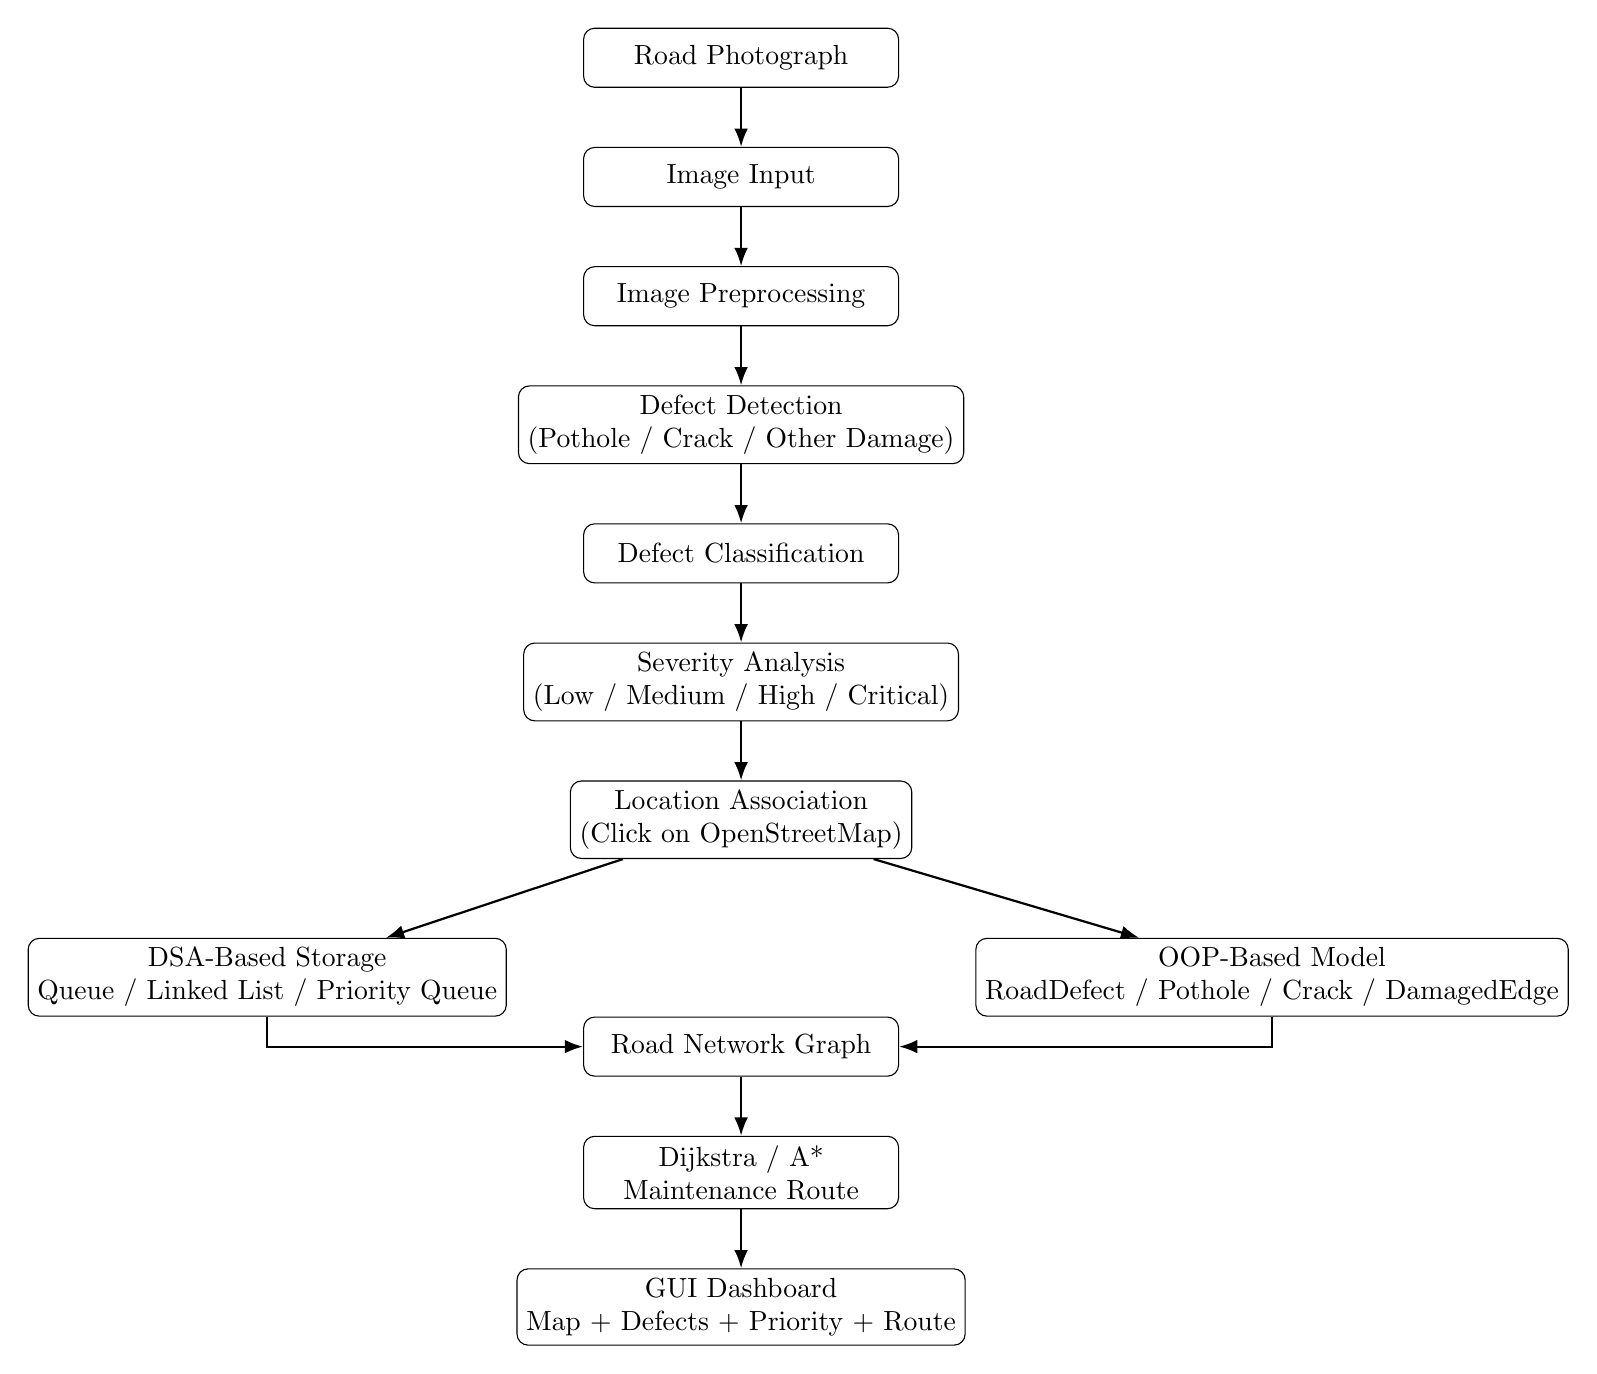
\begin{tikzpicture}[
    node distance=0.75cm,
    box/.style={rectangle, draw, rounded corners, align=center, minimum width=4.0cm, minimum height=0.75cm},
    arrow/.style={-{Latex}, thick}
]
\node[box] (photo) {Road Photograph};
\node[box, below=of photo] (input) {Image Input};
\node[box, below=of input] (prep) {Image Preprocessing};
\node[box, below=of prep] (detect) {Defect Detection\\(Pothole / Crack / Other Damage)};
\node[box, below=of detect] (class) {Defect Classification};
\node[box, below=of class] (severity) {Severity Analysis\\(Low / Medium / High / Critical)};
\node[box, below=of severity] (location) {Location Association\\(Click on OpenStreetMap)};
\node[box, below left=1cm and 0.8cm of location] (dsa) {DSA-Based Storage\\Queue / Linked List / Priority Queue};
\node[box, below right=1cm and 0.8cm of location] (oop) {OOP-Based Model\\RoadDefect / Pothole / Crack / DamagedEdge};
\node[box, below=2cm of location] (graph) {Road Network Graph};
\node[box, below=of graph] (route) {Dijkstra / A*\\Maintenance Route};
\node[box, below=of route] (gui) {GUI Dashboard\\Map + Defects + Priority + Route};

\draw[arrow] (photo) -- (input);
\draw[arrow] (input) -- (prep);
\draw[arrow] (prep) -- (detect);
\draw[arrow] (detect) -- (class);
\draw[arrow] (class) -- (severity);
\draw[arrow] (severity) -- (location);
\draw[arrow] (location) -- (dsa);
\draw[arrow] (location) -- (oop);
\draw[arrow] (dsa) |- (graph);
\draw[arrow] (oop) |- (graph);
\draw[arrow] (graph) -- (route);
\draw[arrow] (route) -- (gui);
\end{tikzpicture}
\end{center}

\section{Map-Based Road Condition Monitoring}

One of the main features of the proposed system is a 2D map of a selected geographical area using OpenStreetMap data. The project can be demonstrated using a particular campus, locality or nearby road network.

OpenStreetMap provides the underlying geographical road map, while the application adds its own defect markers and road-condition information. Leaflet can be used as the interactive map layer for displaying the map, placing markers and handling user clicks.

A typical interaction will be:

\begin{center}
\textbf{Upload Photo}
$\rightarrow$
\textbf{Open Map}
$\rightarrow$
\textbf{Click Exact Defect Location}
$\rightarrow$
\textbf{Capture Latitude/Longitude}
$\rightarrow$
\textbf{Generate/Assign Defect ID}
$\rightarrow$
\textbf{Save Record}
\end{center}

The application can use custom coloured markers:
\begin{itemize}[leftmargin=*]
    \item \textbf{Green:} Good/Normal road condition
    \item \textbf{Yellow:} Moderate condition
    \item \textbf{Orange:} High-severity defect
    \item \textbf{Red:} Critical/Poor condition
\end{itemize}

When the user selects a marker, the system can display:
\begin{itemize}[leftmargin=*]
    \item Defect ID
    \item Defect Type
    \item Severity
    \item Road Name/ID
    \item Latitude and Longitude
    \item Repair Status
    \item Option to View the Corresponding Photo
\end{itemize}

The map markers are application-level data placed over the OpenStreetMap base map. The OpenStreetMap map itself does not determine whether a road has a pothole; SmartRoad stores and displays that information.

For the prototype, the map area may be predefined. The project should also display appropriate OpenStreetMap attribution and follow the applicable tile usage requirements.

\section{Application of Data Structures and Algorithms}

\subsection{Queue}

A Queue follows FIFO (First In, First Out). It can store incoming road images waiting to be processed.

\subsection{Linked List}

A Linked List can maintain the history of detected road defects. Each node may store defect ID, type, severity, location, image reference and repair status.

\subsection{Priority Queue / Heap}

A Priority Queue organizes repair tasks based on severity, allowing urgent defects to be considered first.

\subsection{Graph}

The road network is represented using a weighted Graph:
\begin{itemize}[leftmargin=*]
    \item Vertices/Nodes = Intersections or locations
    \item Edges = Roads
    \item Edge Weight = Distance or travel cost
\end{itemize}

\subsection{Dijkstra / A*}

Dijkstra's algorithm or A* can find a shortest or low-cost route between the maintenance depot and selected defect locations.

\subsection{Searching and Sorting}

Searching can find a defect by ID, type, road or status. Sorting can arrange defects according to severity, size or priority.

\section{Application of Object-Oriented Programming}

\subsection{Abstraction}

A general \texttt{RoadDefect} class can define important operations such as severity calculation and displaying details without exposing unnecessary implementation details.

\subsection{Encapsulation}

Attributes such as defect type, severity, location and repair status are kept inside the class and accessed through suitable member functions.

\subsection{Inheritance}

A common base class \texttt{RoadDefect} can have derived classes:
\begin{verbatim}
RoadDefect
   |-- Pothole
   |-- Crack
   |-- DamagedEdge
\end{verbatim}

\subsection{Polymorphism}

A function such as \texttt{calculateSeverity()} can behave differently for different defect classes.

\section{System Architecture}

The system consists of:
\begin{enumerate}[leftmargin=*]
    \item Image Input Module
    \item Image Processing Module
    \item Defect Detection Module
    \item Severity Analysis Module
    \item OOP Defect Management Module
    \item DSA Management Module
    \item OpenStreetMap/Leaflet Map and Road Graph Module
    \item Route Planning Module
    \item GUI Dashboard
\end{enumerate}

Overall architecture:

\begin{center}
\textbf{Road Photos}
$\rightarrow$
\textbf{Image Processing}
$\rightarrow$
\textbf{Defect Detection}
$\rightarrow$
\textbf{Severity + Location}
$\rightarrow$
\textbf{DSA/OOP}
$\rightarrow$
\textbf{Repair Priority}
$\rightarrow$
\textbf{Road Graph}
$\rightarrow$
\textbf{Dijkstra/A*}
$\rightarrow$
\textbf{GUI + OpenStreetMap}
\end{center}

\section{Technology Stack}

\begin{itemize}[leftmargin=*]
    \item \textbf{C:} DSA implementation.
    \item \textbf{C++:} OOP and application logic.
    \item \textbf{OpenCV or equivalent:} Image processing and computer vision.
    \item \textbf{GTK or another suitable desktop GUI framework:} GUI development.
    \item \textbf{OpenStreetMap:} Real-world map data/base map.
    \item \textbf{Leaflet:} Interactive map display, markers and map-click handling.
    \item \textbf{Dijkstra/A*:} Route planning.
    \item \textbf{VS Code, GCC, G++ and Git/GitHub:} Development tools.
\end{itemize}

\section{Methodology}

\begin{longtable}{p{0.12\textwidth} p{0.78\textwidth}}
\toprule
\textbf{Week} & \textbf{Activity} \\
\midrule
1 & Requirement Analysis: Identify requirements, input format, defect categories, map requirements and expected outputs. \\
2 & Image Collection: Collect road photographs containing potholes, cracks and other visible defects. \\
3 & Image Processing: Apply preprocessing operations. \\
4 & Defect Detection: Identify candidate damaged regions. \\
5 & OOP Implementation: Create RoadDefect and derived classes. \\
6 & DSA Implementation: Implement Queue, Linked List, Priority Queue and Graph. \\
7 & Map Integration: Integrate the OpenStreetMap-based map, enable location selection and associate defect locations with coordinates. \\
8 & Route Planning: Use Dijkstra or A* to calculate a suitable maintenance route. \\
9 & GUI Integration: Combine image display, defect records, map, priority information and route output. \\
10 & Testing: Test image processing, classification, severity, DSA operations, map marking and route calculation. \\
\bottomrule
\end{longtable}

\section{Expected Outcome}

The final system is expected to provide a working prototype in which a user can upload road photographs and obtain structured information about road conditions.

The application will be able to:
\begin{itemize}[leftmargin=*]
    \item Process road photographs.
    \item Identify visible road defects.
    \item Classify defect types.
    \item Estimate severity.
    \item Associate defects with exact road locations.
    \item Mark road conditions on an OpenStreetMap-based 2D map.
    \item Maintain defect history.
    \item Prioritize repair tasks.
    \item Represent the road network as a graph.
    \item Suggest suitable maintenance routes.
    \item Display results through a GUI.
    \item Allow a map marker to show the corresponding defect information and photograph.
\end{itemize}

\section{Project Deliverables}

\begin{enumerate}[leftmargin=*]
    \item SmartRoad application.
    \item Image-processing and defect-detection module.
    \item DSA modules in C.
    \item OOP modules in C++.
    \item OpenStreetMap-based 2D road-condition map.
    \item Interactive defect-location marking.
    \item Road-defect data management.
    \item Priority-based repair management.
    \item Graph-based route-planning module.
    \item GUI dashboard.
    \item Sample road-image dataset.
    \item Testing results.
    \item Project report and presentation.
    \item Final project demonstration.
\end{enumerate}

\section{Assumptions}

\begin{itemize}[leftmargin=*]
    \item Road defects are sufficiently visible in input photographs.
    \item Images have reasonable resolution and lighting.
    \item The prototype initially supports a predefined set of defect categories.
    \item Severity can be estimated using predefined rules or image-analysis features.
    \item Location can initially be selected manually on the OpenStreetMap-based map.
    \item The selected map area is predefined for the prototype.
    \item The project is an academic prototype and does not replace professional civil-engineering inspection.
\end{itemize}

\section{Limitations}

Image-based defect detection may be affected by poor lighting, rain or water, shadows, blurred images, low-resolution photographs, different camera angles, occluded defects and similar-looking road textures. Detection accuracy will depend on the quality and diversity of the dataset and the selected detection technique.

The accuracy of the manually selected map location will also depend on the user's map selection. The prototype will initially use a predefined geographical area and may not provide complete live-road information.

\section{Future Scope}

\begin{enumerate}[leftmargin=*]
    \item Integrate AI/deep-learning models for improved pothole and crack detection.
    \item Automatically obtain GPS coordinates from the device or image metadata.
    \item Improve OpenStreetMap integration with detailed road geometry and location markers.
    \item Store repeated observations and monitor road deterioration over time.
    \item Generate optimized routes for multiple high-priority repair locations.
    \item Add database support for large numbers of images and defect records.
    \item Add cloud-based access for maintenance teams.
    \item Use historical data for predictive road maintenance.
\end{enumerate}

\section{Conclusion}

SmartRoad is an image-based road-condition monitoring and maintenance-prioritization system that uses road photographs instead of dedicated physical sensors. It combines image processing with DSA, OOP, graph algorithms and GUI development.

The system detects visible road defects, estimates their severity, associates them with exact locations and displays them on an OpenStreetMap-based 2D map. Users can select a defect location directly on the map, after which the latitude and longitude are stored with the corresponding defect record and photograph. DSA structures provide efficient organization and prioritization of defects, while OOP provides a modular representation of different road-defect types. Graph algorithms enable maintenance-route planning.

The proposed project provides a practical implementation of computer-science concepts in a real-world infrastructure problem and can later be extended with AI-based detection, automatic GPS, richer OpenStreetMap integration, databases and predictive maintenance.

\section{References}

\begin{enumerate}[leftmargin=*]
    \item T. H. Cormen, C. E. Leiserson, R. L. Rivest and C. Stein, \textit{Introduction to Algorithms}, MIT Press.
    \item E. Balagurusamy, \textit{Object Oriented Programming with C++}.
    \item OpenCV Documentation -- Image Processing and Computer Vision.
    \item Leaflet Documentation -- Interactive Maps and Map Markers.
    \item OpenStreetMap Foundation -- OpenStreetMap Data and Tile Usage Policies.
    \item Research literature on automated pothole and crack detection using computer vision.
    \item Research literature on graph-based shortest-path algorithms and road-network optimization.
\end{enumerate}

\end{document}
